\section{\texorpdfstring{Samoopravne a perfektni kody, Lloydova veta}{Samoopravne a perfektni kody, Lloydova veta}}

\vspace{5mm}
\large

\begin{definition}
	Necht A je konecna mnozina (abcda), $q = |A|$. Na mnozine slov $w \in A^n, |w| = n$ definujme Hammingovu metriku jako pocet pismen ve kterych se lisi
	\[ d_H(x, y) = |\{i : x_i \neq y_i \}| \]

	Libovolnou $C \subseteq A^n$ nezyvame kodem delky n nad abcdeou o q symbolech. C opravuje t chyb, pokud
	\[ d_H(x, y) > 2t + 1 \]

	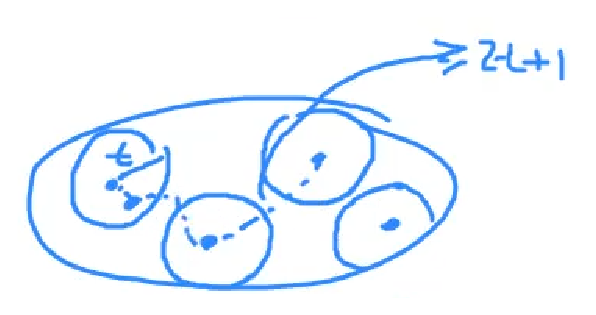
\includegraphics[scale=0.5]{code_1.eps}
\end{definition}

\begin{observation}
	Pokud vezmeme graf vsech slov delky n, hrany povedou mezi 2 slova ktere se lisi presne v 1 souradnice. Pak grafova vzdalenost je prave Hammingova metrika. Na druhou stranu tento graf je n-ta kartezska mocnina grafu o q vrcholech.

	Kod C opravuje t chyb $\iff$ okoli kodovych slov o polomeru t jsou po 2 dizjunktni.
\end{observation}

\begin{observation}
	Kartezsky hrana $\times$ hrana je $\square$.
\end{observation}

\begin{definition}
	\[ \Gamma(n,q) = (A^n, \{xy: d_H(x, y) = 1 \}) = K_q^n \]
\end{definition}

\begin{note}
	Pokud kod C opravuje t chyb, pak
	\[ |C| \leq \frac{q^n}{\sum_0^t \binom{n}{i} (q - 1)^i} \]

	Vezmeme okoli bodu x polomeru t:
	\[ |N_{\Gamma}(x)| = 1 + n(q - 1) + ... = \]
	Kde 1 je vrchol sam, pak mame n pozic na kazde muze dojit k $(q - 1)$ chybam.
	\[ = \frac{q^n}{\sum_0^t \binom{n}{i} (q - 1)^i} \]
	binom odpovida zpusobum zvolit pismeno. $(q - 1)^i$ je pocet chyb.

	Pak nerovnice pro velikost C je \# vsech slov deleno velikosti okoli.

\end{note}

\begin{definition}
	Kod je t-perfektni, prave kdyz $|C| > 1$, C opravuje t chyb a nastava rovnost.
	\[ |C| = \frac{q^n}{\sum_0^t \binom{n}{i} (q - 1)^i} \]

	Cely graf je pokryty okoli o polomeru t. Vyuzivaji beze zbytku cely graf (kodova slova).
\end{definition}

\begin{note}
	Perfektni kody skoro neexistuji.

	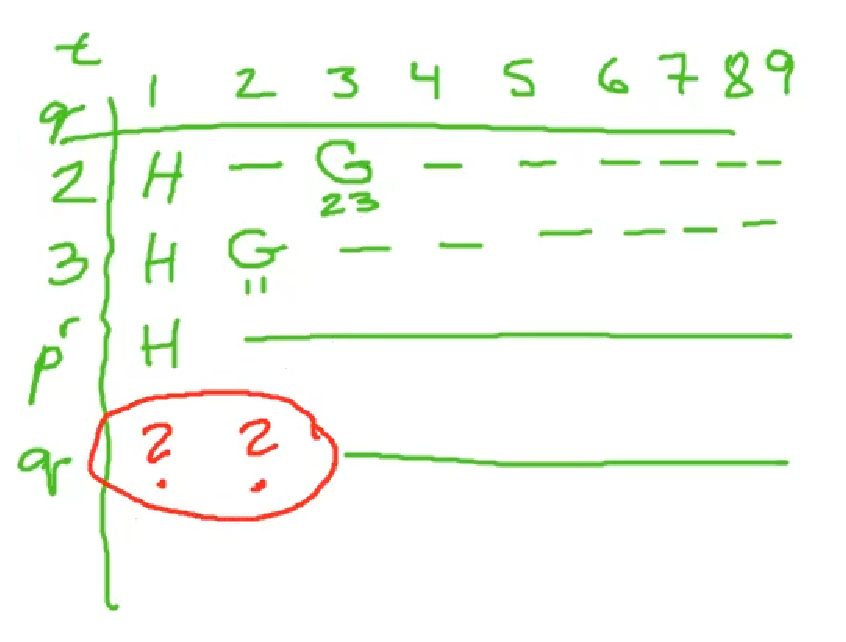
\includegraphics[scale=0.5]{code_2.eps}
\end{note}

\begin{observation}
	pro $q = p^r$, C je t-perfektni kod delky n.
	\[ |C| = \frac{q^n}{\sum_0^t \binom{n}{i} (q - 1)^i} \in \Z \]

	Pak suma v jmenovateli deli $q^n = p^{rm}$. Takze i suma je mocnina p. Dokazeme ze suma se rovna $q^l, l \in \N$.

\end{observation}

\begin{proof}
	\[ \sum_0^t \binom{n}{i} (q - 1)^i = q^a p^b = p^{ra + b}, 0 \geq b < r \]

	Upravime sumu
	\begin{gather*}
	1 + \sum_1^t \binom{n}{i} (q - 1)^i = p^{ra + b}\\
	(q - 1)\sum_1^t \binom{n}{i} (q - 1)^{i - 1} = p^{ra + b} - 1\\
	\sum_1^t \binom{n}{i} (q - 1)^{i - 1} = \frac{q^ap^b - 1}{q - 1} = \frac{q^ap^b - p^b + p^b - 1}{q - 1} = p^b \frac{q^a - 1}{q - 1} + \frac{p^b - 1}{p^r - 1}
	\end{gather*}

	Pak $\frac{q^a - 1}{q - 1} \in \Z$ jako soucet geom rady. Druhy zlomek ale $\in (0, 1)$. Coz dava dohromady cele cislo pouze $b = 0$.
\end{proof}

\begin{theorem}[Hammingovy kody]
	Necht $q = p^r$. Pak 1-perfektni kod delky n nad abcdou o 1 symbolech existuje $\iff n = \frac{q^k - 1}{q - 1}, k \in \N$.

	Coz dostaneme dosazenim $t = 1$ do rovnice minuleho pozorovaji:
	\[ 1 + n(q - 1) = q^k \Rightarrow n = \frac{q^k - 1}{q - 1} \]
\end{theorem}
	Necht $C \subseteq \Z_q^n$. Sestavime matici $H \in \Z_q^{k \times n}$ tak, aby sloupce byly po 2 lin. nezavisle.

	V kazde slozce muzeme vzit $q^k$ symbolu. Nulovy vektor pouzivat nemuzeme. Dohromady $(q^k - 1)$ vektoru. Vezmeme nejaky vektor, linearne zavisle s nim jsou jeho nasobky skalarem krome 0 - $(q - 1)$. Proto
	\[ n = \frac{q^k - 1}{q - 1} \]

	Podivame se na $Ker(H) \subseteq \Z_q^n$. Vime
	\[ \dim(Ker(H)) = n - rank(H) = n - k \]

	Tvrdime, ze v jadru jsou vektory ktere maji vzdalenost aspon 3. Pokud by existovali vektory vzdalenosti 2. Jejich rozdil $\in Ker(H)$.
	Dostali bychom vektor y ktery ma nejvyse 2 nenulove souradnice. Po vynasobeni $Hy$ dostali bychom lin. kombinace 2 vektoru ktere jsou dle volby lin. nezavisle.

	\[ |C| = q^{n - k} = \frac{q^n}{q^k} = \frac{q^n}{1 + n(q-1)} \]
\begin{proof}
\end{proof}

\begin{theorem}[Prvociselne perf. kody(BD)]
	pro $q = p^r$ neexistuji perfektni kody jinych parametru nez Hammingovy, Golayovy (a opakovaci kod s parametry $q = 2, n = 2t + 1$, ktery je povazovan za trivialni).
\end{theorem}

\begin{theorem}[Prvociselne perf. kody $t \geq 3$ (BD)]
	pro $q = p^r$ neexistuji zadne t-perfektni kody opravujici $t \geq 3$ chyb.
\end{theorem}

\begin{theorem}[Lloyd]
	Pokud existuje t-perfektni kod delky n nad abcedou o q symbolech, pak polynom:
	\[ L_t(x) = \sum_{j = 0}^t = (-1)^j(q - 1)^{t - j} \binom{x - 1}{j} \binom{n - x}{t - j} \]

	ma t ruznych kladnych celociselnych korenu mensich nez n. Je to polynom stupne t.

	Myslenka dukazu: najdeme 2 koreny od sebe vzdalene min nez 1. Pak nemuzou byt celociselne.

	Pro $t = 1,2$ umime koreny najit, takze Lloydova veta je prilis slaba.
\end{theorem}
\begin{proof}
	TODO predn 9 od 34:00
\end{proof}

\begin{lemma}
\end{lemma}
\begin{proof}
\end{proof}
